\documentclass{article}
\usepackage{graphicx}
\usepackage[utf8]{inputenc}
\usepackage{float}
\usepackage{hyperref}
\usepackage{booktabs}
\usepackage[margin=1in]{geometry}
\usepackage{booktabs}
\usepackage{booktabs}
\usepackage{subcaption}
\linespread{1.5}
\hypersetup{
    colorlinks=true,
    linkcolor=blue,
    filecolor=magenta,      
    urlcolor=cyan,
    citecolor=cyan
}



\urlstyle{same}


\begin{document}

\title{CoRNonCOB App Note
	   \medskip \large}
\author{Ayesha Ahmad, Ethan Holleman}

\maketitle

\newpage

\section{Abstract}
CoRNonCOB (Compare Really Non-Conserved Oligopeptides in Bacteria) is a tool that identifies peptides in the non-coding regions of bacterial genomes that may contribute to a phenotype of interest. CornNonCOB is designed to work at the very specific scale of individual phenotypes of specific strains of bacteria and because of this RNA-seq data that could illuminate the expression profiles of the bacteria of interest may not be available. Therefore, CornNonCOB attempts to leverage genomic data by identifying peptides in non-coding regions that are conserved in the members of a positive phenotype and absent in a control. With this tool, we hope to identify the peptides that are unique to \emph{Lactobacillus crispatus} that produce a microbial agent to kill E. Coli bacteria. Through identifying these unique peptides, we hope to provide another parameter to characterize phenotypes. Our tool takes x amount of genomes in FASTA format  from each phenotype, and generates the peptides unique to each respective phenotype. Our tool is available at the \href{ https://github.com/EthanHolleman/CoRNonCOB}{GitHub page here}, where additional information on the parameters required and our current analyses can be found. Documentation is available at the \href{https://ethanholleman.github.io/CoRNonCOB/index.html}{CornOnCOB website.}

\section{Introduction}
Currently, there are no tools for identifying peptides located in the non-coding regions of bacterial genomes. There are tools that identify peptides in other organisms like plants. For example, the Small Peptide Alignment Discovery Application (SPADA), is an application to identify the small peptides in plant genomes. SPADA uses homology-based modeling to predict peptides that are one to two exons in length. Unfortunately, SPADA is not equipped to handle bacterial genomes because their genomes do not consist of introns \cite{zhou_silverstein_gao_walton_nallu_guhlin_young_2013}.
\\

There is a database that stores the current known antimicrobial peptides called the Antimicrobial Peptide Database (APD). APD has aided in classifying Antimicrobial Peptides (AMP) and identifying peptides with similar sequences \cite{wang_2004}. AMPs are peptides associated with the ability to kill bacteria, viruses and fungi \cite{izadpanah}. CoRNonCOB is designed to identify peptides in the noncoding regions of bacterial genomes. For this specific project, we are looking at \emph{L. crispatus.} \emph{L. crispatus} are associated with a healthy vaginal and urinary tract microbiome environment \cite{becknell_spencer_2015}. In fact, Lactobacillus probiotics have been found to prevent recurrent Urinary Tract Infections (UTIs) in women \cite{dwyer_dwyer_2012}.
\\

There are two phenotypes of L. jensenii that we hope to distinguish by identifying unique peptides. One phenotype characterized by their ability to produce a microbial agent to kill E. Coli, while the other phenotype does not appear to produce any agent to kill E. Coli. With CoRNONCOB we hope to identify if there are any AMPs in the L. jensenii that show characteristics of killing E.Coli. 


\section{Implementation}

\subsection{Workflow}
CornOnCob is written in python and incorporates Prokka for prokaryotic gene prediction, BioPython for sequence translation and IO, the CD-HIT suite of programs for sequence clustering and the modelamp package for chemical property
calculations. The generalized workflow can be seen in figure \ref{fig:flow}.
\\

\begin{figure}[h]
\centering
\includegraphics[width=12cm]{/home/ethan/Documents/github/CoRNonCOB/sphinx/images/diagram.png}
\caption{Histogram of candidate peptide properties identified from Putoni Lab \emph{Lactobacillus crispatus} genomes vs. all AMPs available from the \href{http://aps.unmc.edu/AP/main.php}{AMP3 Database}.}
\label{fig:flow}
\end{figure}
The user supplies paths to directories containing the genomes of the members of each phenotype. Running prokka on each genome produces a gff file of predicted coding regions which CornOnCob then reads and inverts to yield predicted non-coding regions for each genome. Non-coding regions are translated into all six reading frames, written as fasta files in the program output. These fasta files representing the predicted non-coding peptides from individual genomes are then concatenated to create a file containing the predicted non-coding peptides of an entire phenotype. CD-HIT is then used to cluster the concatenated non-coding peptide files by sequence similarity. CD-HIT uses a greedy algorithm that sorts sequences by length and then searches for similar sequences via kmer comparison allowing for extremely fast sequence clustering \cite{10.1093/bioinformatics/btl158}. The longest sequence in each cluster is considered the representative sequence for that cluster. The user can control the minimum overlap of subject to representative sequence and minimum identify thresholds in the CoRNonCOB arguments. 
\\

Peptide clusters meeting a certain threshold of genome participation are considered conserved and written to a new fasta file representing the predicted conserved non-coding peptides for an individual phenotype. CD-HIT-2D, which uses the same basic algorithm of CD-HIT but looks for peptides in one library that are similar to another library, compares the conserved non-coding peptides between the two phenotypes. CoRNonCOB then parses this output and removes non-unique sequences to produce a fasta file of candidate peptides that are uniquely conserved in the positive phenotype. Lastly, using the modelamp python package basic chemical properties of each peptide are predicted and written to a csv file.

\subsection{Run Time and Memory Usage Estimates}


\begin{figure}[H]
  \centering
  \begin{minipage}[b]{0.45\textwidth}
    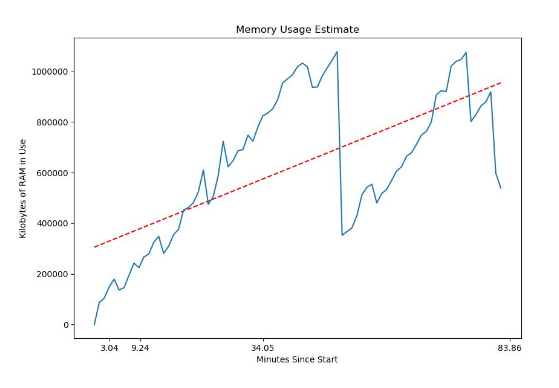
\includegraphics[width=\textwidth]{/home/ethan/Documents/github/CoRNonCOB/sphinx/images/memory.png}
    \caption{CoRNonCOB Memory usage with increasing numbers of genomes.}
    \label{fig:memory}
  \end{minipage}
  \hfill
  \begin{minipage}[b]{0.4\textwidth}
    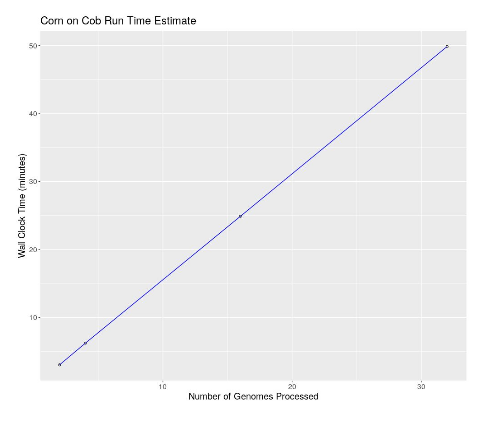
\includegraphics[width=\textwidth]{/home/ethan/Documents/github/CoRNonCOB/sphinx/images/O.png}
    \caption{CoRNonCOB wallclock runtime with increasing numbers of genomes.}
    \label{fig:runtime}
  \end{minipage}
\end{figure}

Figure \ref{fig:runtime} shows the time for CoRNonCOB to execute given an increasing number of genomes. All of the genomes used were of similar length. With this metric CoRNonCOB appears to run in linear time. Operations performed in python by CoRNonCOB such as non-coding region extraction and translation are done in linear time with respect to number of genomes and number of non-coding regions. 
\\


However, Prokka is by far the rate limiting step in CoRNonCOB’s runtime which is estimated as O(n\textsuperscript{2}) where n is the length of the genome used for prediction. Therefore if genome size remains relatively constant, runtime will reflect figure \ref{fig:runtime} but will increase to O(n\textsuperscript{2}) as genome size increases. Memory usage is estimated approximately O(n) where n is the number of genomes processed. The memory usage for the runs shown in figure \ref{fig:runtime} are plotted in figure \ref{fig:memory}.


\section{Results} 

Using CoRNonCOB in test mode and with the bacterial genomes provided from the Putonti Lab and the University of Wisconsin. In order to test the performance of CoRNonCOB we created a collection of 18 experimentally verified AMPs and randomly divided the peptides into positive or negative tests. Positive test peptides were randomly inserted into noncoding regions of only the positive genomes while negative test peptides were inserted into all genomes. This is shown in the table below.\ref{tab:prefom}.


\begin{table}[H]
\centering
\begin{tabular}{@{}lllll@{}}
\toprule
\textbf{Test Type} &
  \textbf{Peptides in Test} &
  \textbf{\begin{tabular}[c]{@{}l@{}}Peptides Expected\\ in Final Results\end{tabular}} &
  \textbf{\begin{tabular}[c]{@{}l@{}}Peptides in\\ Final Results\end{tabular}} &
  \textbf{Percent Correctness} \\ \midrule
Positive &
  9 &
  9 &
  7 &
  77 \\
Negative &
  9 &
  0 &
  0 &
  100 \\ \bottomrule
\end{tabular}
\label{tab:prefom}
\end{table}

Currently, the CoRNonCOB pipeline has been able to recover seven of the nine positive peptides and filter out nine of the nine negative test peptides. Additionally our test run returned a total of 2293 candidate non-coding peptides unique to the positive (\emph{E. coli} lethal) phenotype. Figure \ref{fig:hist} shows histograms comparing properties of the candidates to all peptides in the AMP3 database. 


\begin{figure}[h]
\centering
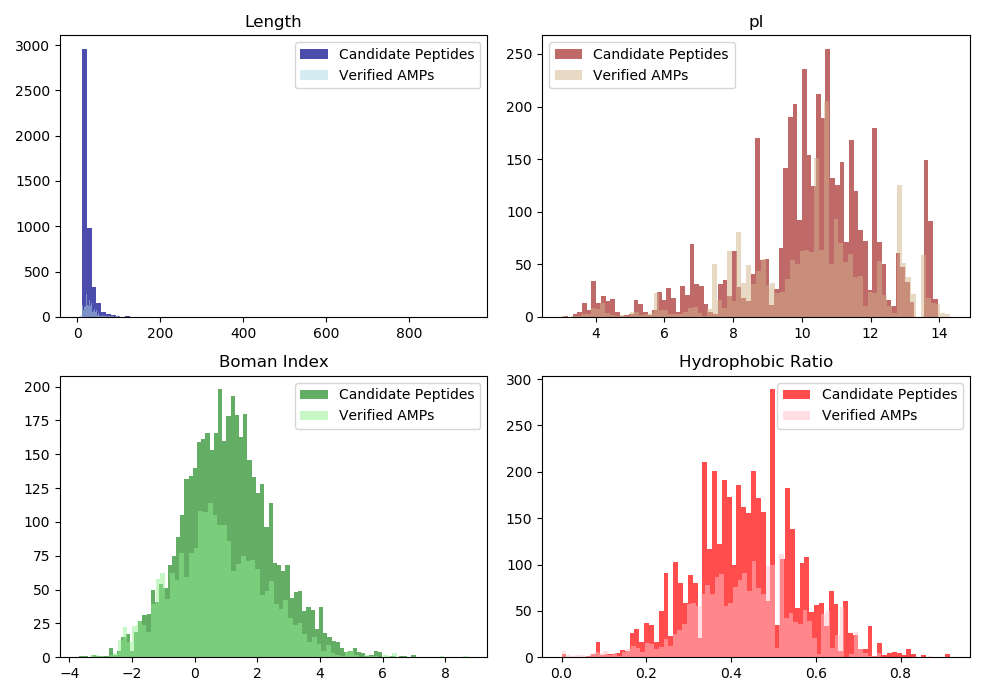
\includegraphics[width=13cm]{/home/ethan/Documents/github/CoRNonCOB/sphinx/images/pep_props.png}
\caption{Histogram of candidate peptide properties identified from Putoni Lab \emph{Lactobacillus crispatus} genomes vs. all AMPs available from the \href{http://aps.unmc.edu/AP/main.php}{AMP3 Database}. Length is in amino acids. The Boman index is a measure of potential for protein-protein interaction \cite{boman_2003}. Hydrophobic ratio is ratio of hydrophobic amino acids over number of amino acids in the peptide.}
\label{fig:hist}
\end{figure}

We have also reached out to the Sheshu lab at George Mason university to obtain the source code for their AMP classification model described in their 2018 publication Deep learning improves antimicrobial peptide recognition in order to try and narrow down the candidate peptides in the final fasta output.\cite{duchrow_shtatland_guettler_pivovarov_kramer_weissleder_2009}

\newpage
\bibliography{refs.bib}{}
\bibliographystyle{plain}

\end{document}